\documentclass[11pt]{article}
%Gummi|061|=)
\usepackage[table]{xcolor} 
\usepackage{vmargin}
\usepackage[T1]{fontenc} %encoding del font
\usepackage[utf8]{inputenc} %encoding dell'input
\usepackage[italian]{babel} %lingua per la formattazione
\usepackage{mparhack}
\usepackage{pgfplotstable}
\usepackage{float}
%pacchetti per la formattazione
\usepackage{calc} %fantasmi

\usepackage{graphicx} %inserire immagini (grafici vettoriali.pdf)
%pacchetti -->\SCfigure \SCtable
\usepackage{booktabs} %pacchetto per per le tabelle
\usepackage{amsmath, amssymb} %pacchetti per usare comandi matematici
\usepackage{pgf,tikz}
\usepackage{caption}
\usepackage{siunitx}
\usepackage{setspace}
\usepackage{subfig}
\usepackage{array}
\usepackage{multirow}
\usepackage{pgfplots}

\usepackage{graphicx}
\begin{document}

\begin{center}

% Upper part of the page. The '~' is needed because \\
% only works if a paragraph has started.
% \includegraphics[width=0.20\textwidth]{./Logo1}~\\[1cm]

%\textsc{\LARGE University of Trento}\\[1.5cm]

\textsc{\Huge Esperienza II}\\[0.5cm]
%\vspace{30pt}

%\HRule \\[0.4cm]
%\vspace{15pt}
%{ \huge \bfseries Svuotamento di un volume}\\[0.4cm]
%\vspace{15pt}
%\HRule \\[1.5cm]
%\vspace{30pt}
% Author and supervisor


\large
\title{ESPERIENZA 3}

%\emph{\large\textbf{Autori}}\\ \\ 
Michele \textsc{Pedrotti}\\
Luigi \textsc{Bassini}\\
Nicola \textsc{Trevisson}\\
Giacomo \textsc{Alberini}
\\
\vspace{10pt}
\today





\end{center}

\setmarginsrb{30mm}{10mm}{25mm}{10mm}%
             {0mm}{10mm}{0mm}{10mm}


\section{Introduzione}
Scopo dell'esperienza è quello di misurare (in un intervallo che va da $40\ensuremath{^\circ}C$ a $85\ensuremath{^\circ}C$) la pressione di vapore dell'acqua all'equilibrio. Si è cercato, inoltre, di dimostrare la validità dell'equazione di Clausius-Clapeyron che descrive la dipendenza che intercorre tra temperatura e pressione di vapore all'equilibrio.
Una volta verificata la validità della legge si è determinato un valore medio dell'entalpia di vaporizzazione dell'acqua.

\section{Pressione di vapore dell'acqua}

Per le misurazioni di pressione di vapore dell'acqua all'equilibrio abbiamo seguito un particolare procedimento con lo scopo di diminuire, se non eliminare, l'errore sistematico dovuto alla non termalizzazione del tubo in plastica che collega il manometro differenziale alla bottiglia.
Il primo passo consiste nel portare il sistema (una bottiglia da 100 ml riempita per 3/4 di acqua demineralizzata all'interno di un becker più grande contenente acqua e ghiaccio) ad una temperatura di $11^\circ C$. Una volta raggiunto l'equilibrio termico si è proceduto allo svuotamento del volume d'aria dalla bottiglia per poi immergere il condotto che la collega al barometro nell'acqua in essa contenuta. In questa maniera, ripristinando la pressione atmosferica all'interno della bottiglia, il tubo e il barometro si sono riempiti di acqua. Così facendo è possibile ottenere una misura diretta della pressione di vapore dell'acqua contenuta all'interno della bottiglia non influenzata dalle diverse condizioni termodinamiche dell'aria contenuta nel condotto.
 

Abbiamo quindi misurato la pressione di vapore al variare della temperatura. Poiché la relazione supposta tra le due grandezze è del tipo: P $\propto$ exp(T) abbiamo deciso di servirci di un grafico che presentasse sull'asse delle ascisse l'inverso della temperatura assoluta e su quella delle ordinate il logaritmo naturale della pressione. In questo modo la relazione precedente diventa del tipo: ln(P) $\propto$ T, la quale ha l'andamento di una retta.\\
Di seguito riportiamo il grafico ottenuto dai dati rilevati sperimentalmente.

\begin{figure}[H]
\hspace{-38mm}
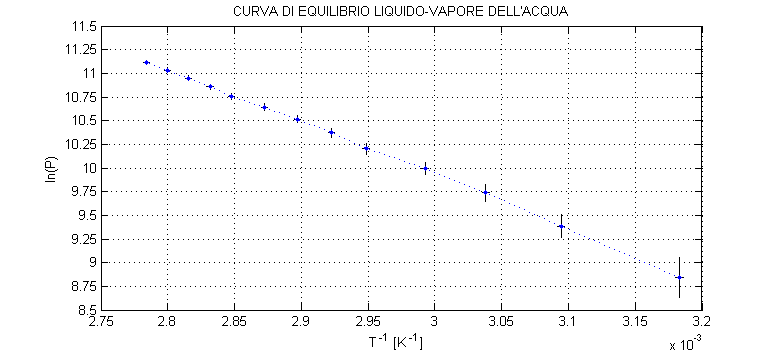
\includegraphics[scale=1.10]{pressione_temperatura.png}
\caption{}
\label{}
\end{figure}

Nel grafico abbiamo riportato anche le barre d'errore relative alle misure effettuate, che aumentano sensibilmente al diminuire dalla pressione. Ciò è giustificato dal fatto che: $\delta$ln(P) $\propto$ $P^{-1}$. Notiamo inoltre che, come ipotizzato precedentemente, i dati rappresentano un andamento lineare.\\
Successivamente, tramite regressione lineare, abbiamo dunque calcolato i parametri di tale retta. 
\begin{center}
\begin{tabular}{|c|c|c|c|}
\hline
a & $\delta$a & b [\unit{K}] & $\delta$b [\unit{K}]\\
\hline
 26.3 & 0.4 & -5.4 $\cdot$ 10$^{3}$ & 2 $\cdot$ 10$^{2}$ \\
\hline
\end{tabular}
\end{center}
Dove a e b rappresentano rispettivamente l'intercetta e il coefficiente angolare della retta. Per verificare la validità di tale legge abbiamo effettuato il test del chi quadro:2
\begin{equation}
X^2 = 1 \pm 4
\end{equation}
Il risultato ottenuto è decisamente minore rispetto al valore atteso del chi quadro, che era di circa 11. Teoricamente un valore così inferiore al chi quadro atteso è indice di una sovrastima delle incertezze sulla pressione. Questa sovrastima è dovuta al fatto che sebbene la risoluzione del manometro differenziale Bourdon in  nostra dotazione fosse moltao bassa (50 \unit{mbar}) l'effettivo errore a cui sono soggetti i valori di pressione è determinato dalla larghezza della tacca relativa alla misura e non alla distanza tra esse.

\section{Entalpia di vaporizzazione dell'acqua}
Il comportamento di un gas in cui vi sia equilibrio tra due fasi della stessa specie chimica è descritto dalla legge di Clausius-Clapeyron, in cui compare come componente il valore dell'entalpia di vaporizzazione/solidificazione. 
\\
Tale valore può essere ricavato utilizzando i parametri trovati con il fit del grafico,in quanto vale la seguente relazione:
$$\ln{p}= -\frac{\lambda}{R}\cdot\frac{1}{T}$$
$$\lambda =m \cdot R$$
con $m$ coefficiente angolare della retta plottata e R costante universale dei gas. \\
Il valore da noi è ottenuto è:
$$\lambda = 45.4 \pm 1.5 ~\text{kJ}/\text{mol}$$   
\\che è compatibile con i risultati presenti in letteratura. 

\end{document}